% Define block styles
\tikzstyle{decision} = [diamond, draw, fill=blue!20, 
    text width=4.5em, text badly centered, node distance=3cm, inner sep=0pt]
\tikzstyle{block} = [rectangle, draw, fill=blue!20, 
    text width=5em, text centered, minimum height=4em]
\tikzstyle{arrow} = [thick,->,>=stealth]
\tikzstyle{cloud} = [draw, ellipse,fill=red!20, node distance=3cm,
    minimum height=2em]

\section{Vývojový diagram}
Vývojový diagram nesouvisí konkrétně s Pythonem, ale je obecnou součástí programování.\\
Je to (grafický) diagram, který znázorňuje v jakém pořadí se provádí jaké výpočty a kroky programu. Znázorňuje ve kterých místech se program dělí do více větví, podle určitého kritéria (podmínky) a také v jakou chvíli program končí.\\
Vývojový diagram nekreslíme pro konkrétní programovací jazyk - je to obecný zápis (znázornění) průběhu programu či algoritmu. Jeho smyslem je přehledně znázornit \uv{co se děje}. Na základě vývojového diagramu jde obvykle snadno zapsat kód v konkrétním programovacím jazyku.\\

\subsection{Odkazy}
Ve vývojovém diagramu existuje spoustu norem a zvyklostí, existuje jich také několik typů.\\
\url{https://cs.wikipedia.org/wiki/V%C3%BDvojov%C3%BD_diagram}

\subsection{Značky}
Pro naše potřeby postačí zjednodušený vývojový diagam s pouze několika základními značkami.\\
Pro začátek a konec algoritmu použijeme ovál (elipsu). Pro krok algoritmu (výpočet, akci) použijeme obdélník. A pro větvení algoritmu (na základě nějaké podmínky - otázky) použijeme kosodélník.

\begin{figure}[h!]
\centering
\begin{subfigure}[t]{.3\textwidth}
\begin{tikzpicture}
	\node [cloud] (start) {Start};
	\node [cloud, below of=start] (end) {Konec};
	
	\draw [arrow] (start) -- (end);	
\end{tikzpicture}   
\label{diagram:start_end}
\caption{Začátek a konec algoritmu (programu)}
\end{subfigure}
%
\begin{subfigure}[t]{.3\textwidth}
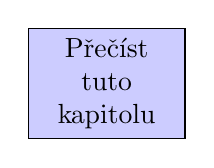
\begin{tikzpicture}
	\node [block] (krok) {Přečíst tuto kapitolu};
\end{tikzpicture}   
\label{diagram:step}
\caption{Jeden krok algoritmu (programu)}
\end{subfigure}
%
\begin{subfigure}[t]{.3\textwidth}
\begin{tikzpicture}
	\node [decision] (podminka) {Chcete se naučit programovat?};
\end{tikzpicture}   
\label{diagram:decision}
\caption{Větvení programu - Podmínka, otázka}
\end{subfigure}
\label{diagram:zakladni}
\caption{Základní značky ve vývojovém diagramu}
\end{figure}

\subsection{Celý diagram}
Ke spojení jednotlivých kroků, resp. míst ve vývojovém diagramu používáme šipky. To můžeme vidět např. na obrázku \ref{diagram:start_end}. Někdy se šipka vrací zpět do určitého místa diagramu (spojuje se s jinou šipkou - spojovací čárou). V takovém případě šipky (čáry) spojíme speciální spojovací značkou (obvykle malým kolečkem), nebo necháme šipku mířit na danou čáru. Nespojujeme čáry v blocích algoritmu. Pokud vedou do bloku algoritmu dvě šipky znamená to, že pro tento krok potřebujeme oba vstupy zároveň (což obvykle není to, co chceme naznačit).

\begin{figure}[h!]
\centering
\begin{tikzpicture}
	\node [cloud] (start) {Start};
	\node [below of=start] (adda) {};
	\node [decision, below of=adda] (chci) {Chcete se naučit programovat?};
	\node [block, right of=chci, node distance=3cm] (motivace) {Najit v sobě motivaci};
	\node [below of=chci, node distance=3cm] (addb) {};	
	\node [block, below of=addb] (cti) {Přečíst tento souhrn.};
	
	\node [decision, below of=cti] (umim) {Už to všechno umím?};	
	\node [cloud, below of=umim] (end) {Konec (spíš teprve pořádný začátek)};
	
	\draw [arrow] (start) -- (chci);
	\draw [arrow] (chci) -- node [near start, below] {ne} (motivace);
	\draw [arrow] (motivace) -- +(0,3) -- (adda);
	\draw [arrow] (chci) -- node [near start, right] {ano} (cti);
	\draw [arrow] (chci) -- (cti);
	\draw [arrow] (cti) -- (umim);
	\draw [arrow] (umim) -- node [near start, below] {ne} +(2,0) -- +(2,4) -- (addb);
	\draw [arrow] (umim) -- node [near start, right] {ano} (end);		
\end{tikzpicture}   
\label{diagram:cely}
\caption{Kompletní ukázka vývojového diagramu}
\end{figure}
 